\chapter{Background}
\label{cha:background}

\begin{comment}
Chapter 2: Background and literature survey
This chapter should give essential background information with references to published material in research papers, books, URLs, magazine articles and even newspapers. Expand on any references to other work that have been mentioned in Chapter 1. Refer to the notes on references (below) for the preferred way of referencing publications. The reader, stimulated by the presentation of ideas in this section, may be led to consult some or all of the referenced publications. This section will be useful for any student in a subsequent year who wishes to take the project further.
\end{comment}

As outlined in \autoref{cha:introduction} the project consists of two major parts: a financial management service, which can be used to view historical spending and gain understanding of personal finances; and a forecasting element which predicts how much spending will occur in the future. 

\section{Statement Management}
There are existing applications that implement similar features to the money management aims of this project\question{Mention the current "bad" internet banking here?} \gavin{Yes}, most notably Lloyds TSB Money Manager, the first and only personal money management application provided by a UK bank and Mint.com a United States (US) only personal finance service \parencite{lloyds2014moneymanager, mint2014whatismint}.

\subsection{Lloyds Money Manager}
The service is available to Lloyds TSB current account holders as part of their online banking and its features revolve around documenting historical spending \parencite{lloyds2014money}.

The key features include:
\begin{itemize}
\item Categorising spending
\item Creating spending plans per category
%\item View dates money came in and out in a calendar
\item Viewing money spent per category
\item Track progress of budget targets
\end{itemize}

Customer reviews of the service highlight the usefulness of spending analysis screen, which includes a breakdown of spending in each \gls{category} (Fig. \ref{fig:moneymanager}, as well as the spending calendar, which displays money spent in a day by day format.
%
The reviews, however, also highlight some shortcomings, noting that changes to categories are not reflected immediately, categories are often incorrect and that it's not possible to override the \gls{category} for a single transaction, for example food bought at a petrol station is placed in the Car \gls{category} and cannot be moved \cite{moneywatch2011lloyds, moneysupermarket2011lloyds}.

\begin{figure}[h]
    \centering
    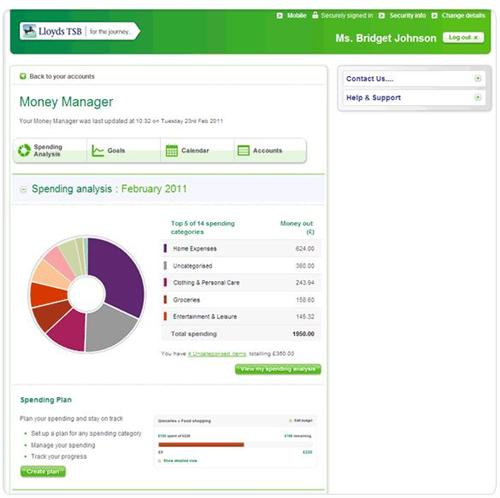
\includegraphics[width=0.8\textwidth]{background/moneymanagerchart}
    \caption[Spending Analysis by category on Lloyds Money Manager]{Spending Analysis by category on Lloyds Money Manager \parencite{lloyds2014money}}
    \label{fig:moneymanager}
\end{figure}

A key advantage of the money manager is that Lloyds already have access to their customer data, so there is no data entry or upload required, which could be confusing and off-putting to potential users.

\subsection{Mint.com}
Mint.com offers very similar features to Lloyds but is limited to the US. However, Mint automatically logs into the users online bank account and downloads their statements authenticating with their banking username and password. It's reported that this feature relies on the use of application programming interface's (API) at each bank which Intuit (the company behind Mint) have negotiated access individually, though Intuit have published no information to support or dispute this \cite{stackoverflow2012bankingapi, stackoverflow2012bankingapi2}.
% 
Although this feature is clearly useful and saves time for the users, it does make Mint responsible for storing their customers Internet banking passwords and presumably involves fee payments to the banks providing these API's.
%
For these reasons it was decided that automatic statement uploading was outside of the budget and scope of this project, however, the project should support manual upload of statements to avoid date entry of users.

\subsection{Mobile Apps}
Mobile applications or `apps' as they are commonly known have seen a surge in popularity since the release of smartphones and are a common target for small pieces of software, such as financial organisation \parencite{purcell2011half}.

The three most popular iPhone personal financial applications \cite{itunes2013topapps}, at the time of planning the project, all offered features very similar to those found in the Lloyds Money Manager and Mint. The most popular features being grouping money by \gls{category} and graphs of spending history.
% 
However, they all had the same drawback, the user had to manually enter all of their transactions and set categories for them, which appears time consuming and error prone, particularly on a mobile app \cite{spendee2014spendee,budgt2013budgt,bluetags2014pocket}.

The increase of mobile usage should be considered when planning the features of the project, with the project ensuring mobile compatibility and if possible, avoiding manual data entry. \plan{This needs improving}

\section{Prediction}
Predicting future transactions before they occur is technically similar to the work done by investors on the stock market, where the objective is to predict whether the value of a stock will fall or increase in order to make buy/sell decisions.

Preifer and Carraway demonstrated that Markov Chain Models can be used to model customer relationships with a business and predict the expected value of a marketing engagement with an individual customer. By creating a transition matrix of a particular customer transitioning from not spending to spending and visa versa over five periods\footnote{An `illustration' assuming a customer will never return after 5 months of not spending}, they were able to estimate the likelihood of a spend occurring in a given period, Fig. \ref{fig:preifermarkovchain} shows a graphical representation of the model that was produced, the states represent the five periods, where $p_{i}$ is the probability of the transition occurring during period $i$ \cite{pfeifer2000modeling}.
% 
The researchers were to calculate the expected loan to value ratio (LTV) for the customer over the periods, by taking a matrix \lorna{of?}costs and gains associated with a purchase in each period and multiplying that by the probability of a purchase occurring taken from the transition matrix. This gives the expected present value for each period, which can be used to decide when to end a relationship with a customer (preventing the costs).
%
They demonstrate the application of Markov Chain Models (MCM) to a larger dataset, calculating the optimal policy for ending relationships with customers depending on varying costs concluding that the use of MCM's is an effective way of making customer relationship decisions. However, this paper assumes the company making predictions already knows how much money a customer will spend during each interaction and is focused around calculating the probability of a spend occurring. An implementation applied to the personal spending space will require a way to predict the value of the future transaction.
{Mention what MCM's are here?} \gavin{Yes, expand on CMC's}

\begin{figure}[h]
    \centering
    %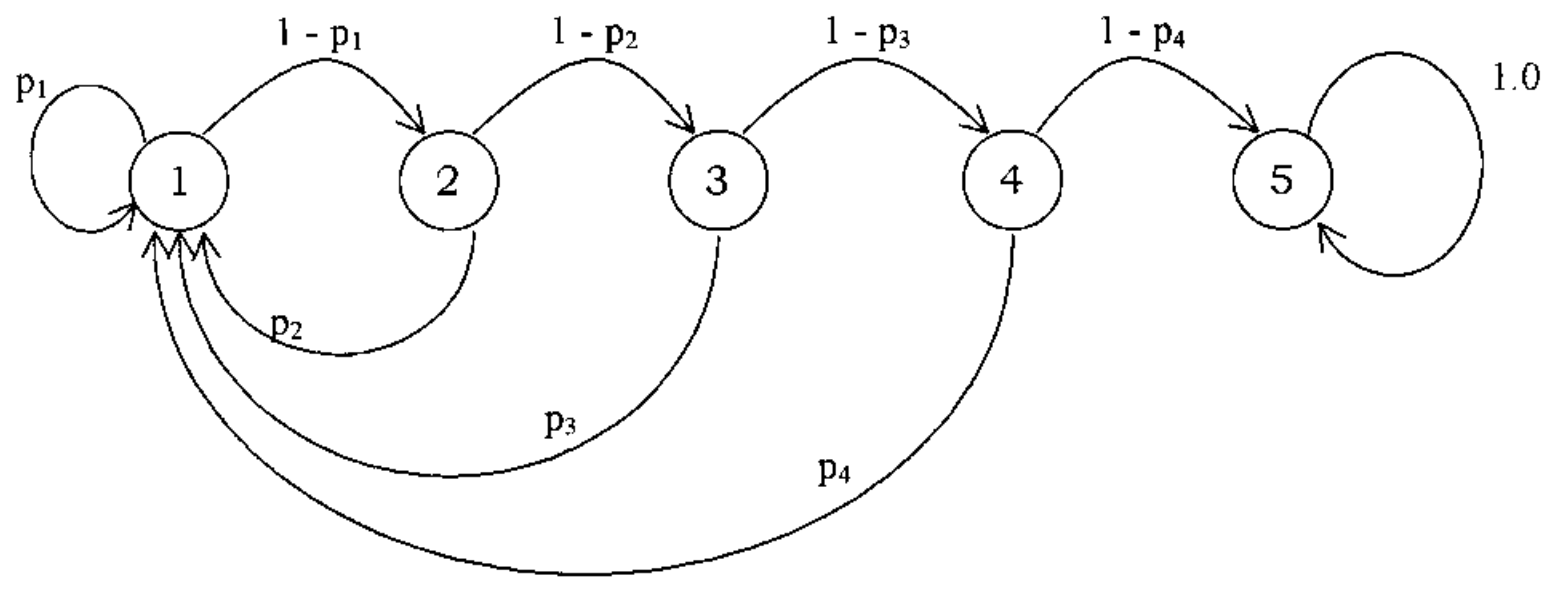
\includegraphics[width=\textwidth]{background/markovchain}
    \begin{tikzpicture}[start chain=going right]
    \node[state, on chain]                 (1) {1};
    \node[state, on chain]                 (2) {2};
    \node[state, on chain]                 (3) {3};
    \node[state, on chain]                 (4) {4};
    \node[state, on chain]                 (5) {5};
    \
    \draw[
        >=latex,
    %   every node/.style={above,midway},% either
        auto=right,                      % or
        loop above/.style={out=75,in=105,loop},
        every loop,
        ]
     (1) 	edge[bend left] node [above]{$1 - p_{1}$}   (2)
      		edge[out=145,in=220,loop,looseness=6]             node {$p_{1}$}   (1)
     (2) 	edge[bend left] node[above]{$1 - p_{2}$}   (3)
      		edge[bend left=90,,in=120]             node {$p_{2}$}   (1)
     (3) 	edge[bend left] node[above] {$1 - p_{2}$}   (4)
     		edge[bend left=90,in=105,]             node {$p_{3}$}   (1)
     (4) 	edge[bend left] node [above]{$1 - p_{2}$}   (5)
     		edge[bend left=90,in=90]             node {$p_{4}$}   (1)
     (5) 	edge[out=40, in=320,loop,looseness=6] node[right]{$1.0$}   (5);
    
    
    % The \draw path is like the one above.
    \end{tikzpicture}
    \caption[Markov Chain Model of customer spending]{Markov Chain Model for a particular customer over five periods \parencite[Adapted from Fig. 1]{pfeifer2000modeling}}
    \label{fig:preifermarkovchain}
\end{figure}

% OTHER PREDICTION
Research by Singh et al., from the Massachusetts Institute of Technology, studied the spending behaviour of 52 adults and investigated the impact of social interactions, including text messages, phone calls and face-to-face meetings, on the participants spending in order to predict their spending behaviour. Using a Na\"{i}ve Bayes classifier and selecting a subset of their available features using an Information Gain approach, choosing those with most relevance to each classification task, they were able to correctly classify whether the participant would overspend, explore a diverse range of businesses and remain loyal to a business with 72\% overall accuracy. They concluded that social factors, were better ``predictors of spending behaviour'' than personality traits, which had been previously studied \parencite{singh2013spendingbehaviour}.
%
Although this paper did not study the affects of the participants previous transactions on spending, they were able to predict the users spending behaviour, highlighting that factors other than the transaction history may be of importance when trying to predict a users future outflow. However, the paper does not attempt to make a prediction of the amount spent or how many transactions occur.

% AVERAGES
Smoothing is typically applied to financial market data, for example the value of a particular stock on the FTSE 100. The most common techniques are simple, weighted and exponential moving averages, which all reduce the noise found in the data potentially revealing an orderly process, by removing outliers found in the data. The result of this effect can be seen in Fig \ref{fig:dashweightedaverages} \parencite{dash2012movingaverages}.

\begin{figure}[h]
    \centering
    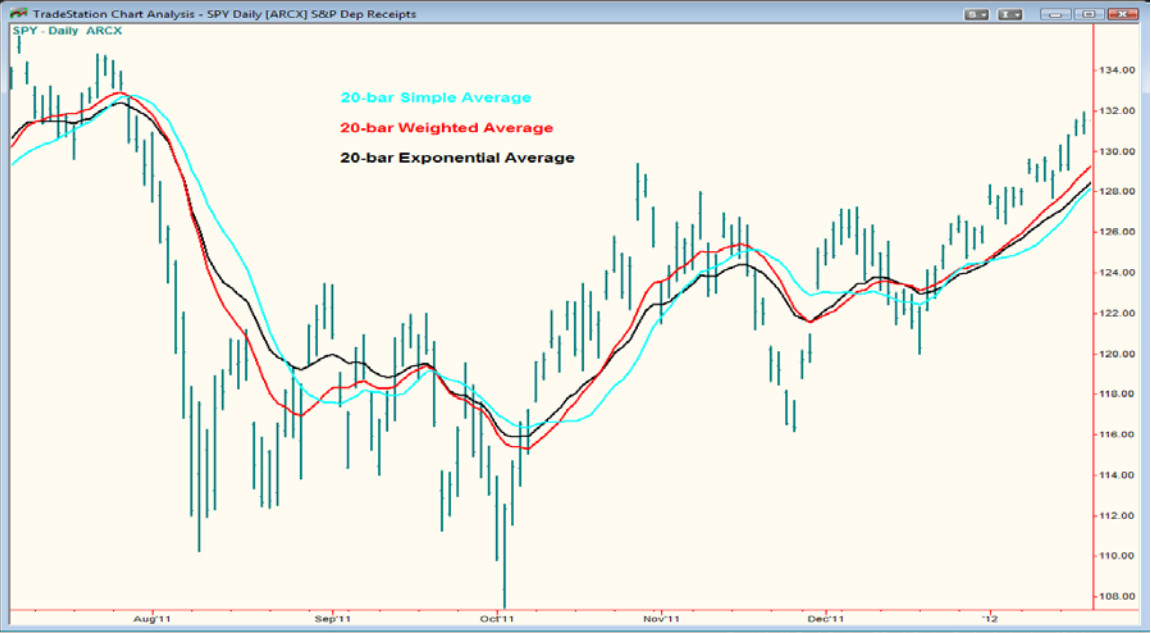
\includegraphics[width=\textwidth]{background/movingaverages}
    \caption[SMA, WMA and EMA of the S\&P500]{Simple Moving Average (MA) [blue], Weighted MA [red] and Exponential MA [black] of the S\&P500\protect\footnotemark  \parencite[Fig. 5]{dash2012movingaverages}}
    \label{fig:dashweightedaverages}
\end{figure}
\footnotetext{A stock market index of 500 American companies, the US equivalent of the FTSE 500}

These techniques can be applied to a discrete set of numerical time series data, such as personal expenditure over time in order to make an estimate of what the next value in the series will be \parencite{filliben2003nist}. A prediction can be made using the formula in Fig. \ref{fig:weightedmeanforumla}, where $w_{i}$ is the weight and $x_i$ is the value at time period $i$. Simple smoothing is the equivalent of $w_i = 1$, while exponential smoothing is based around a negative exponential law such as $w_i = e^{-n+i}$, both are examples of weighted smoothing and the weights can be decided in different ways depending on what is being predicted. Time periods with a higher weight have a greater affect on the mean, so in order to make a future prediction, the most recent time period would have a higher weight.

\begin{figure}[h]
    \centering
    \[
        \frac{w_1 x_1 + w_2 x_2 + \cdots + w_n x_n}{w_1 + w_2 + \cdots + w_n}.
    \]
    \caption{Using weighted smoothing to predict a future value}
    \label{fig:weightedmeanforumla}
\end{figure}

% Holt winters extends smoothing, to take into account trends in data
Smoothing (and therefore prediction) can be extended to take into account trends and possible seasonal fluctuations using double and triple smoothing, respectively. A technique known as `Holt-Winters double exponential smoothing` takes into account trends in data, which single smoothing does perform accurately with, by factoring the weighted average growth between previous the time series when calculating the average for each period \parencite{kalekar2004holtwinters}.
% 
Extending the calculation into double and triple smoothing when estimating a users future outflow was decided as a possible extension for the project. A discussion of this technique can be found in \autoref{section:triplesmoothing}.

\section{Security}
The project stores peoples personally identifiable information and needs to be backed by strong security standards, before designing the project and as part of the ethics application procedure common web security practice was researched.

\subsection{Account Hijacking} \label{subsection:account-hijacking}
On the web, information is sent sent between the users web browser and the remote server over HTTP information in plain text and can easily be read using a man-in-the-middle attack. This risk is compounded if accessing the Internet via an an unencrypted WiFi connection\footnote{Common at Coffee Shops and Universities} which would allow anyone in the local area to `sniff' the information by simply scanning for capturing the transmitted packet.

If a website involves authentication, this becomes a serious security risk. Authentication is usually performed by sending the username and password in plain text to a remote server which is validated, and if valid issuing the user with a session cookie.
%
A potential attacker could observe and store these usernames and passwords, which is why commonly websites such as Facebook use HTTPS for the login, ensuring the usernames and passwords are sent encrypted to the server.

If a website falls back to HTTP following authentication, the risk of unauthorised account access is still prevalent.
%
In order to identify which user the browser is authenticated as it sends a session cookie to the remote server with each request. 
%
Although the attacker can't observe the username and password, the session cookie is being sent in plain text with every request, and the attacker can perform a session hijack by downloading the content of that cookie to their local machine (Fig. \ref{fig:securitysniffing}) and then sending it to the remote server with their HTTP request `proving' they are the user and gaining access to their account (Fig. \ref{fig:securityhijacking}) \parencite{owasp2011sessionhihacking}.
% 
Firesheep was a proof of concept plugin for Firefox released in 2010 that demonstrated this vulnerability, showing that session hijacking could be performed on popular sites including Google, Facebook, Twitter, Dropbox and Flickr, which until recently were not using sitewide SSL to protect their cookies \parencite{butler2010firesheep, butler2014firesheep}. 
%http://codebutler.com/firesheep/ FireSheet mention, http://codebutler.github.io/firesheep/
%
More recently `WhatsApp Sniffer', available on Google Play until May 2012 was able to display messages addressed to other WhatsApp users connected to the same network using this technique \parencite{thehsecurity2012whatsapp}.

\subsection{Password Security}

A common cracking technique used to gain unauthorised access to a user account is a known as a brute force attack. If an attacker knows a particular users username they can perform targeted guessing of the password by enumerating through all possibilities. A websites ability to resist this kind of attack is called the `password guessing resistance'. It is for this reason that many websites enforce password rules in an attempt to increase the number of possible combinations for a password, or the entropy \cite{helkala2008authentication}.

Shannon Entropy can be used estimate the strength of a passwords resistance to this kind of attack. The entropy is calculated using $H(X)= -\sum_{i=1}^n{p(x_i)\log_b p(x_i)}$ where $p(x_i)$ is the probability of the value $x$ occurring \cite{burr2013electronic}.
%
The paper suggests a predefined set of rules for estimating entropy based on Shannon's work studying English text, however other papers found that using this predefined set of rules was not a valid measure of password strength \cite{weir2010shannon}.

\subsection{Database Storage} \label{subsection:databasestorage}
Unfortunately, it is common for the contents of a websites database to be leaked, whether by an administrator of the website or using other techniques such as SQL injection \parencite{bbc2012linkedinpasswords,chechik2013passwords}. It's important to think about the security of the data held within the database, as well as the security of the front end.

If a users password is stored in a reversible state, whether that is plain text or encrypted and the database is leaked, not only can that users account can be accessed on the original website, but the data can be used attack other websites and compromise the users account there, if using the same username and password.
%
Encryption is equivalent to plain text in that, it is simply a case of finding the encryption key, which is very possible using brute force and all the data is in plain text. 
%
This is why standard security practice is to hash passwords. The only way to `decrypt' a hash is to guess the original input by brute force and see if that matches the output.
%
However crackers often make use of Rainbow tables, collections of precalculated hashes and the input used to create them, allowing an attacker to simply lookup a hash in their database to get the result rather than enumerating all the possibilities \parencite{jorgensen2012}.
%
To reduce the effectiveness of this attack method, `salting' is commonly used. Salting involves adding a random collection of numbers and letters to each password. This means that the generated hash is dependent on both the users password and the salt, and therefore a Rainbow Table would need to be generated for each user, cancelling out the advantage of precalculation and making the tables useless \parencite{morris1979password}.
